\documentclass[hyperref={pdfpagelabels=false}]{beamer}

\usepackage{ucs}
\usepackage[utf8x]{inputenc}
\usepackage[T1]{fontenc}
\usepackage[ngerman]{babel}

\usepackage{url}
\usepackage{etoolbox}
\appto\UrlBreaks{\do\a\do\b\do\c\do\d\do\e\do\f\do\g\do\h\do\i\do\j
\do\k\do\l\do\m\do\n\do\o\do\p\do\q\do\r\do\s\do\t\do\u\do\v\do\w
\do\x\do\y\do\z\do\-}

\usepackage{tikz}
\usepackage{lmodern}
\title{Hintergrundsegmentierung}   
\author{Christian Tanzer\\Jonas Bühlmeyer} 
\date{9. Dezember 2016} 



\begin{document}

\begin{frame}
	\maketitle
\end{frame}

\setcounter{framenumber}{0}
\addtobeamertemplate{navigation symbols}{}{
\usebeamerfont{footline}
\usebeamercolor[blue]{footline}
\hspace{1em}
\insertframenumber/\inserttotalframenumber
}


\begin{frame}
	\begin{figure}
		\centering
		\begin{tikzpicture}[scale=0.98]
			\node at (0,0){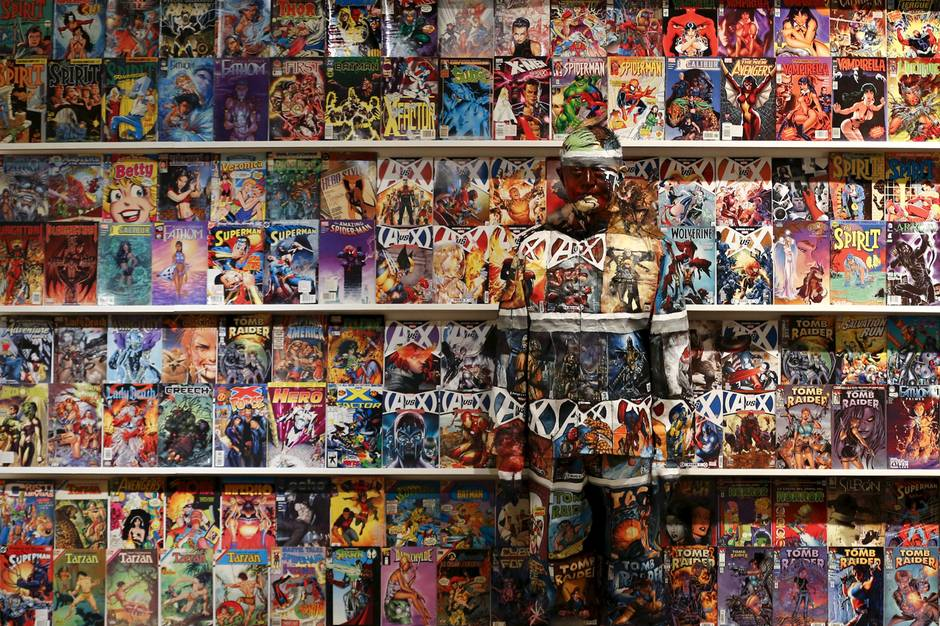
\includegraphics[width=0.98\textwidth]{bilder/einstieg.jpg}};
		\end{tikzpicture}
	\end{figure}
\end{frame}

\begin{frame}
	\begin{figure}
		\centering
		\begin{tikzpicture}[scale=0.98]
			\node at (0,0){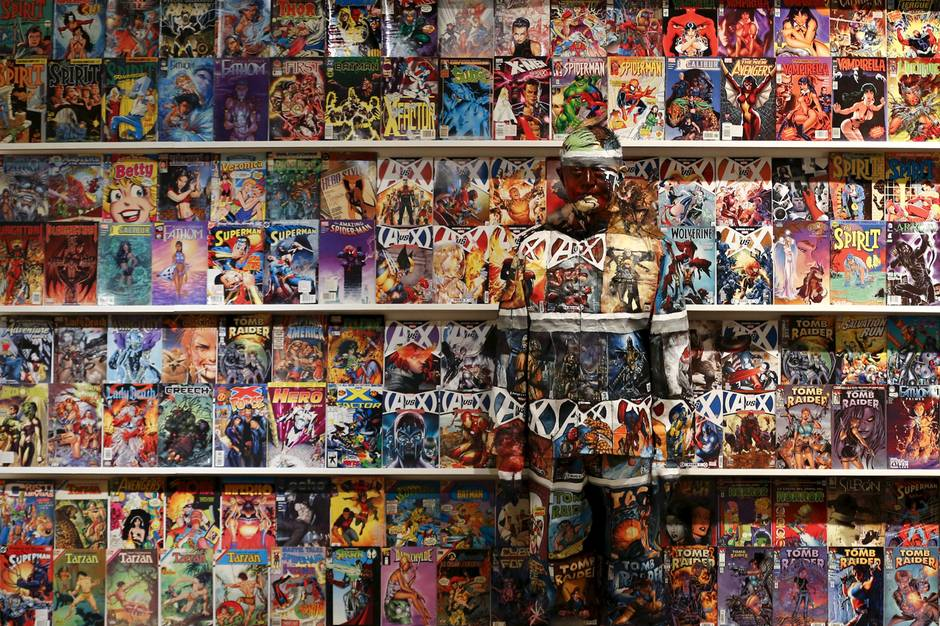
\includegraphics[width=0.98\linewidth]{bilder/einstieg.jpg}};
			\draw[color=white, ultra thick] (0,2.3) rectangle (2.7,-3.5);
		\end{tikzpicture}
	\end{figure}
\end{frame}



\begin{frame}
	\begin{figure}[]
		\centering
		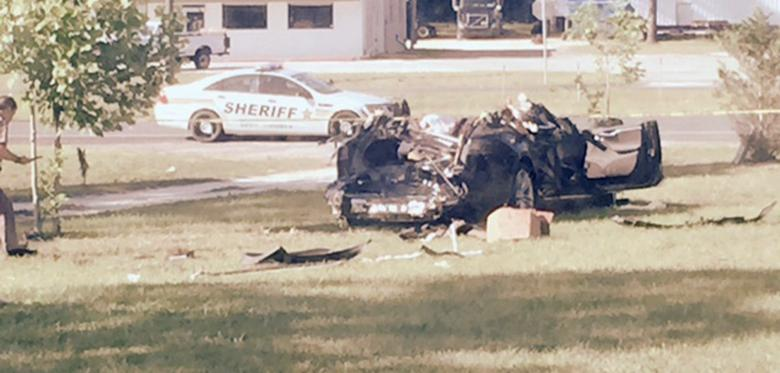
\includegraphics[width=\linewidth]{bilder/tesla.jpg}
		\label{fig:einstieg}
	\end{figure}
\end{frame}


\begin{frame}[t]{Pixelbasiert}
	\begin{figure}[]
		\centering
		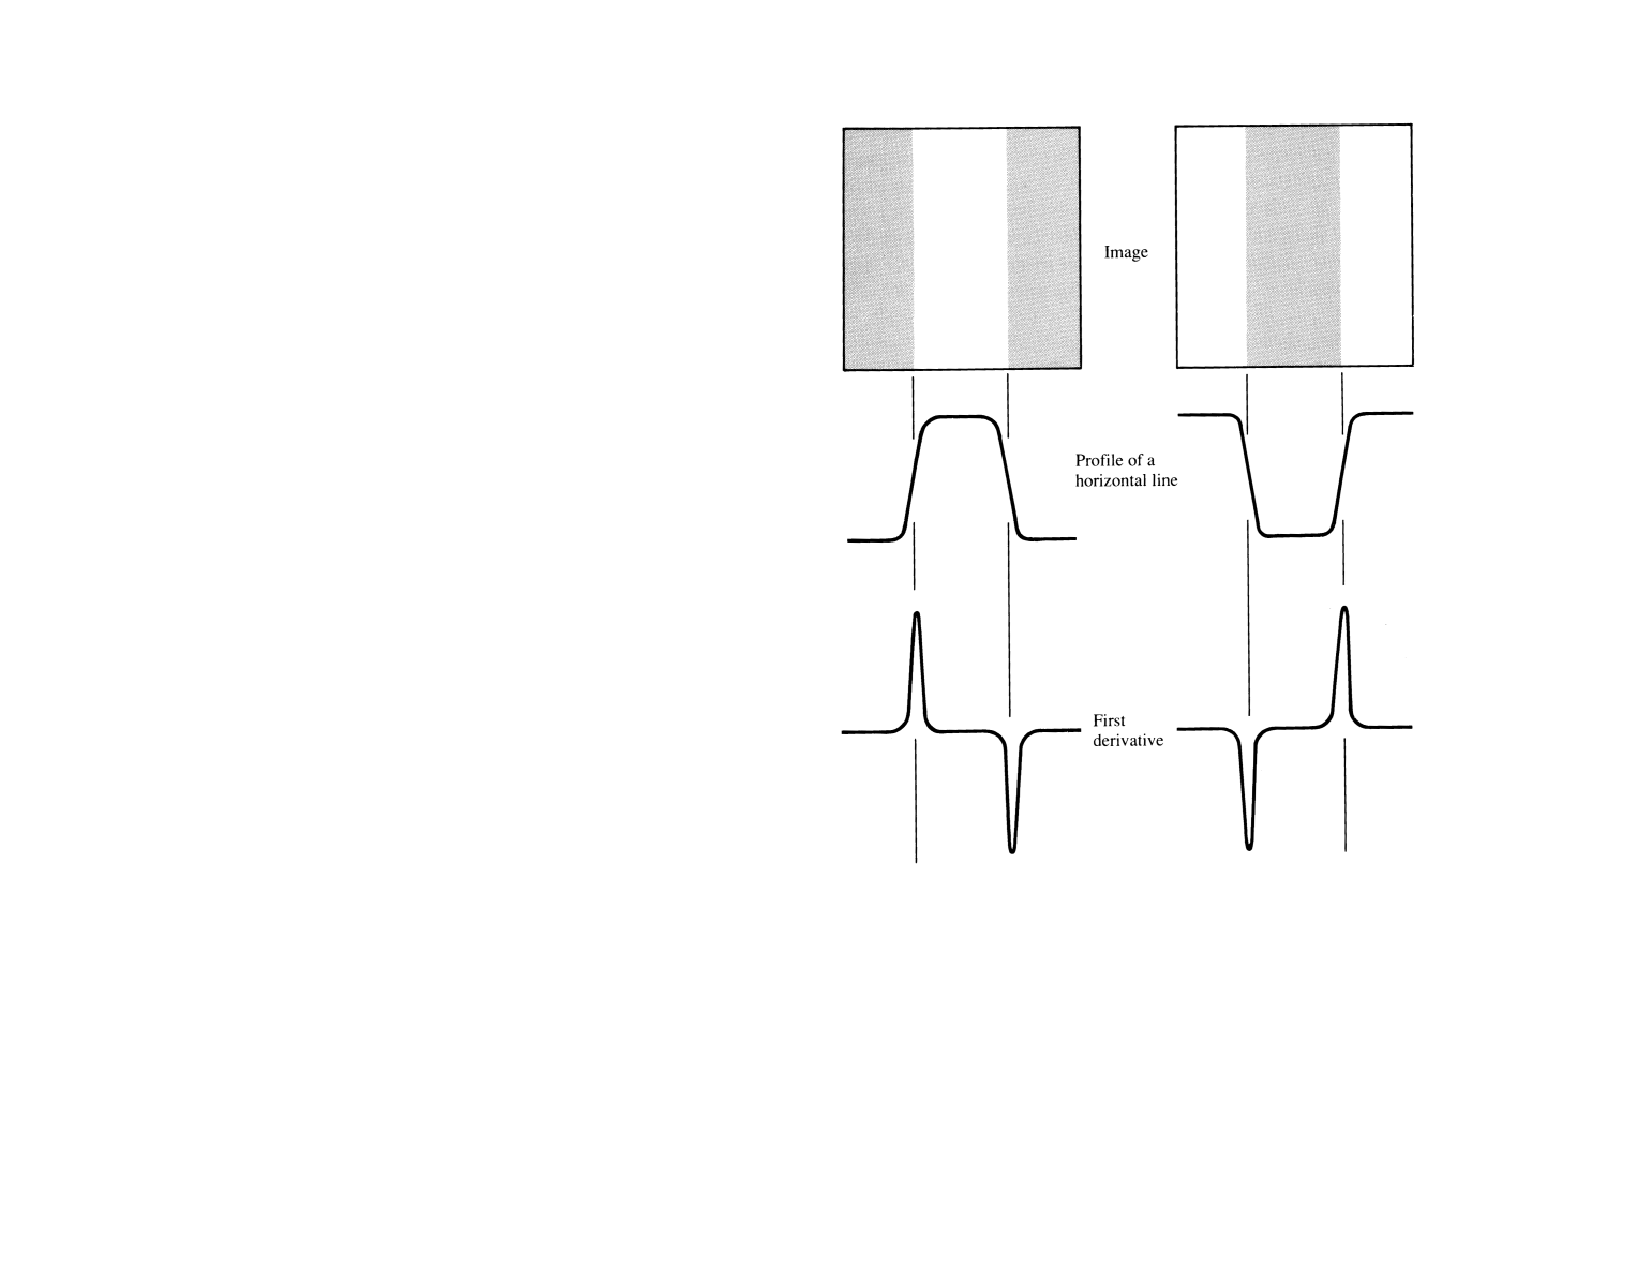
\includegraphics[width=0.55\linewidth]{bilder/pixelbasiert.pdf}
		\label{fig:einstieg}
	\end{figure}
\end{frame}

\begin{frame}[t]{Erkennung von Veränderungen}
	\begin{figure}[]
		\centering
		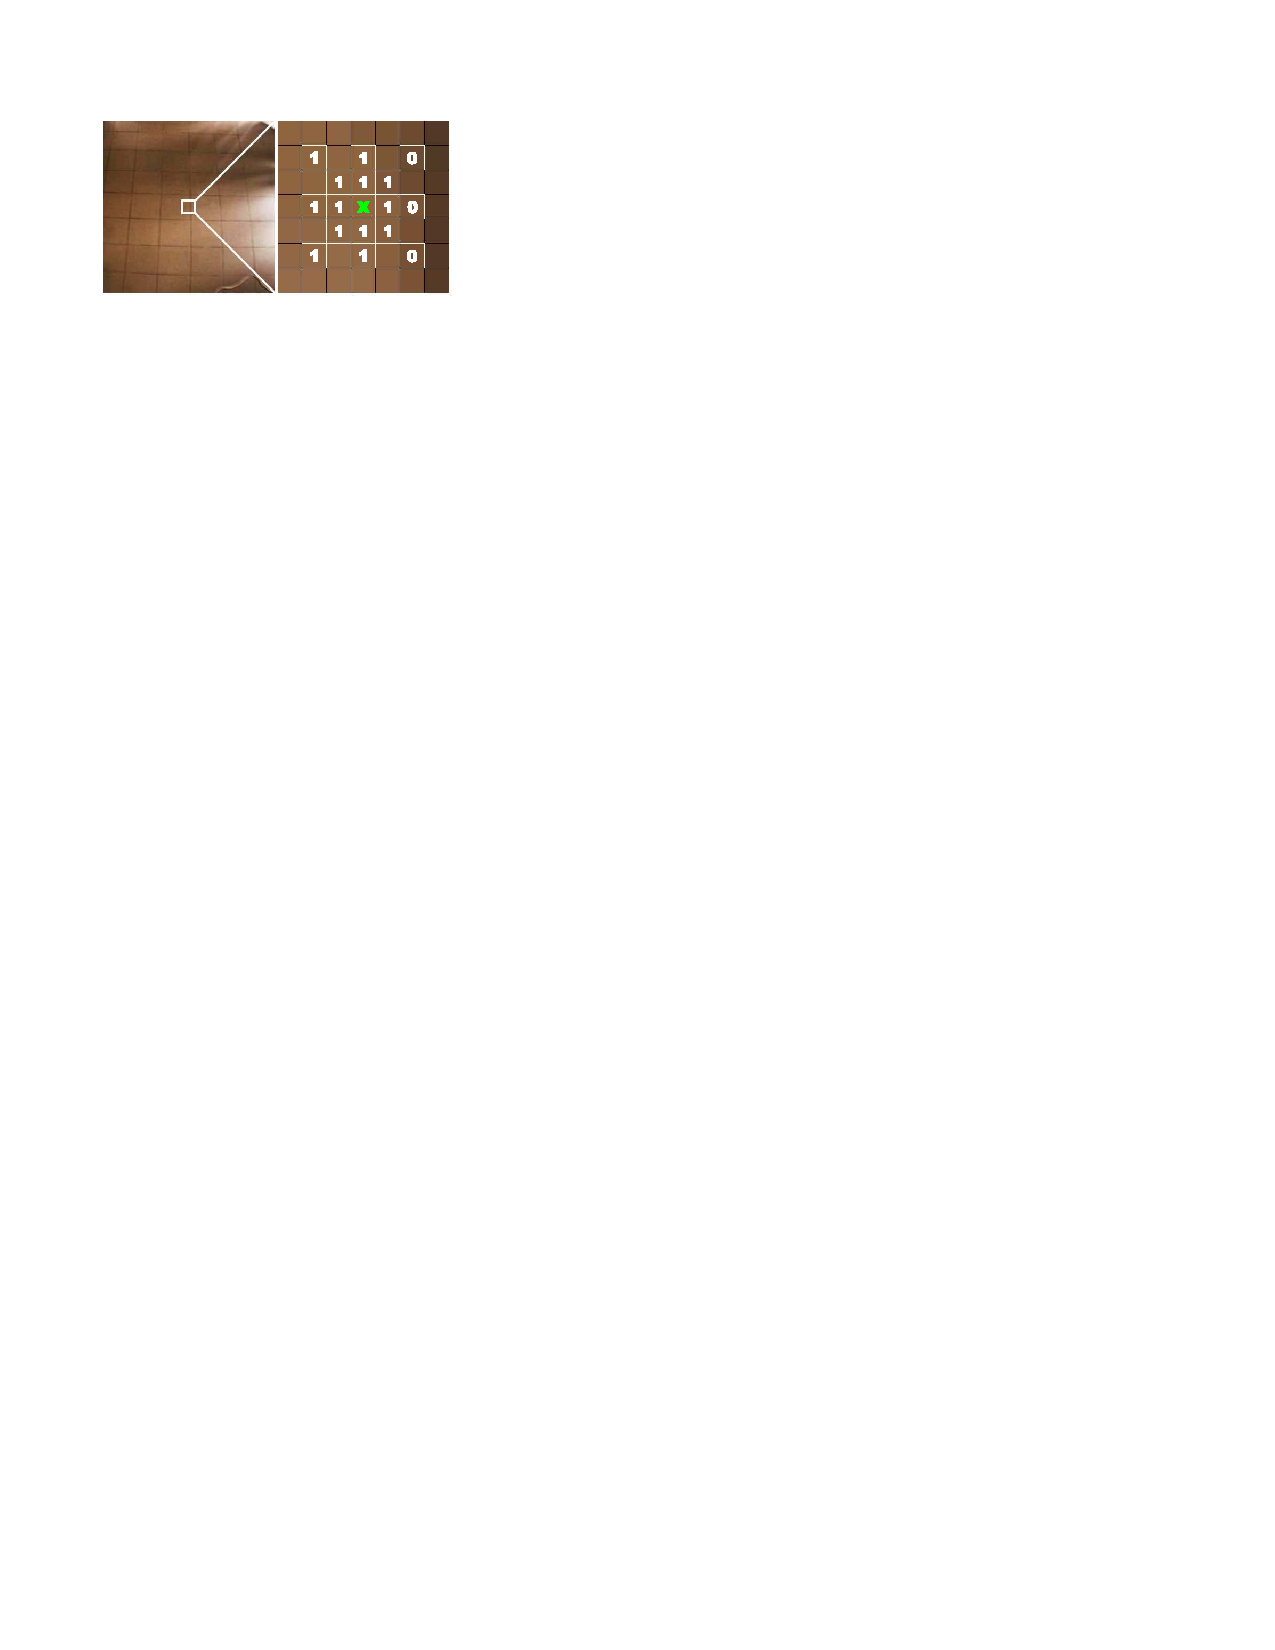
\includegraphics[width=0.55\linewidth]{bilder/change_detection1.pdf}
		
		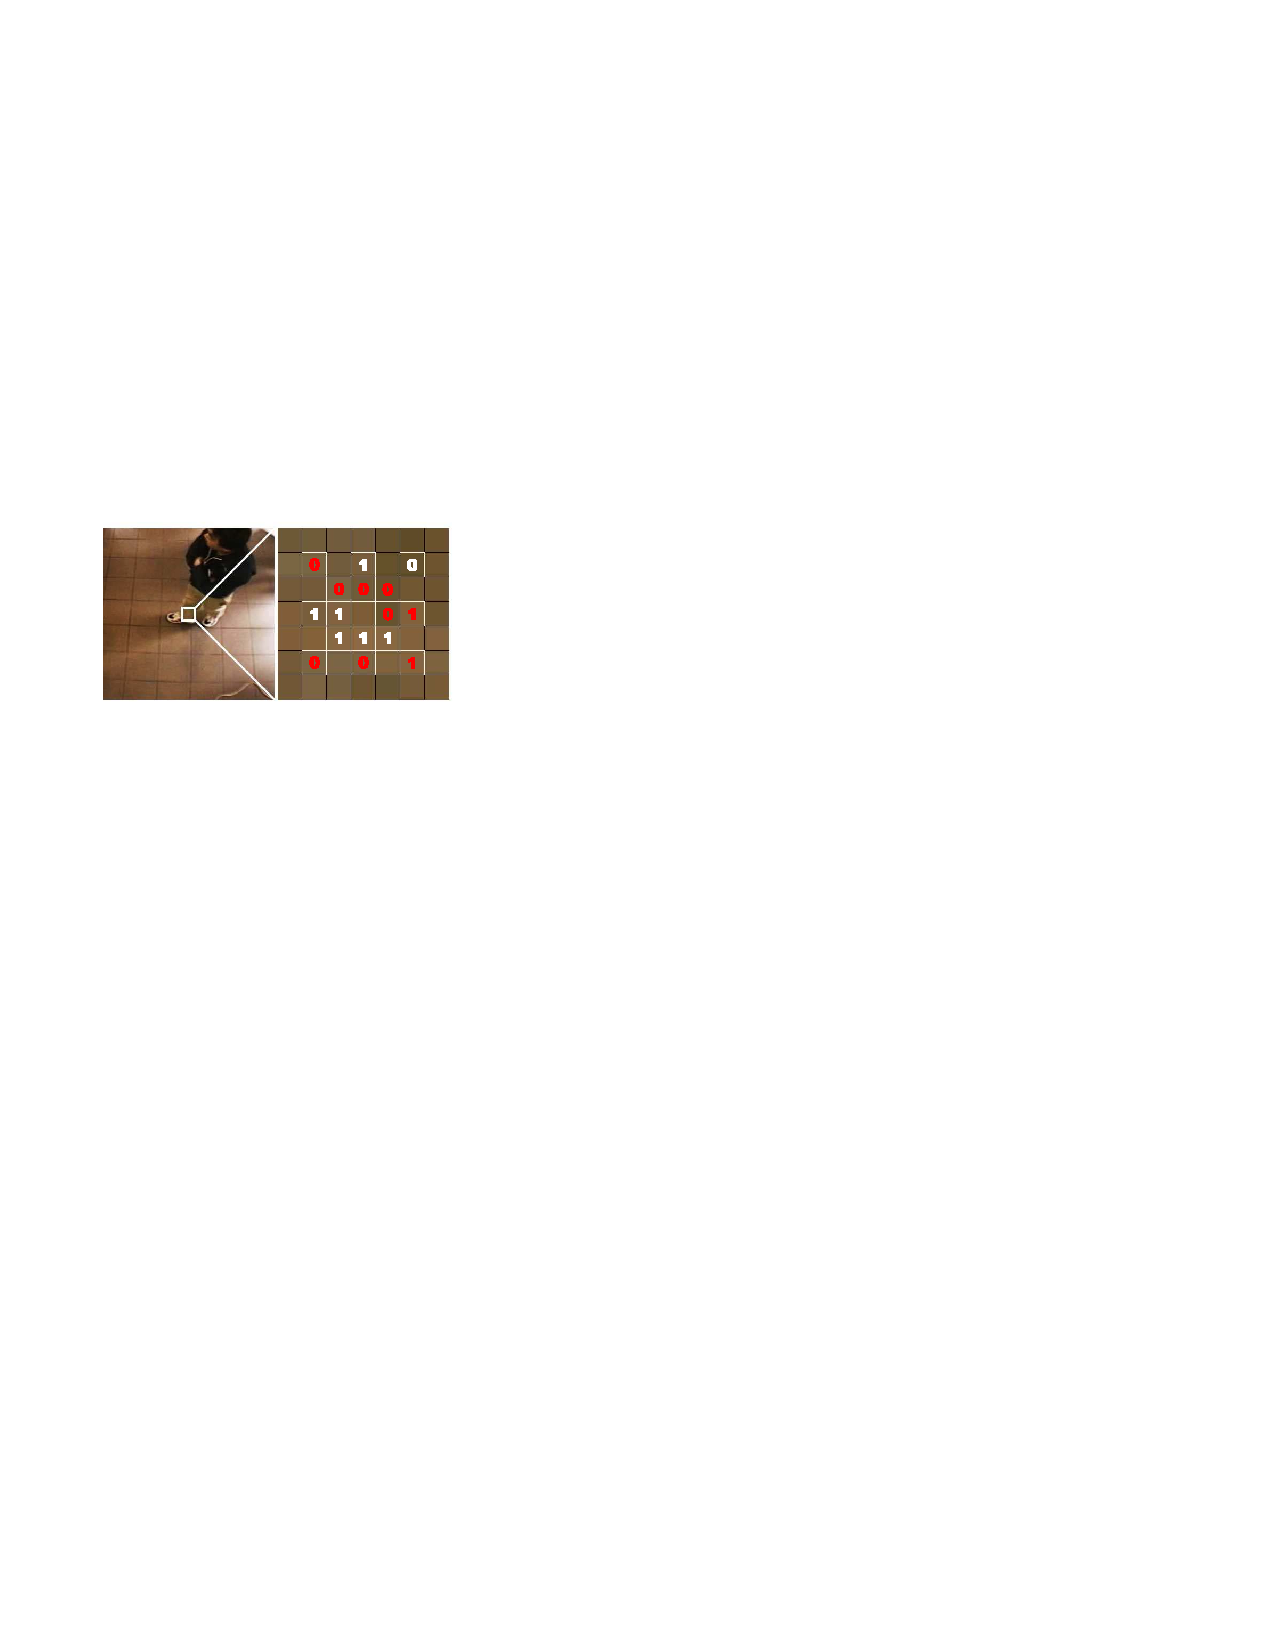
\includegraphics[width=0.55\linewidth]{bilder/change_detection2.pdf}
		\label{fig:einstieg}
	\end{figure}

\end{frame}

\begin{frame}
	\begin{figure}[]
		\centering
		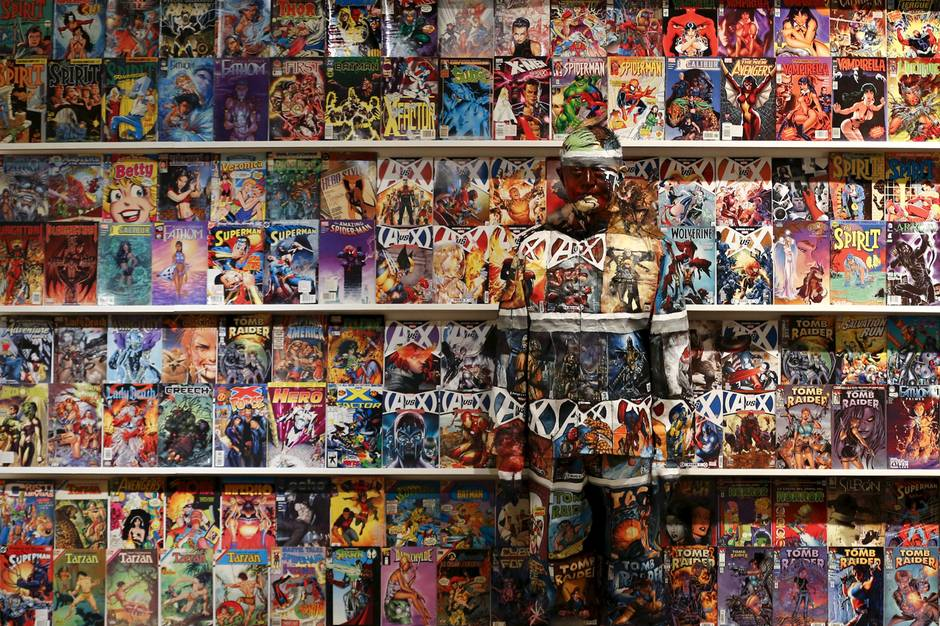
\includegraphics[width=0.98\linewidth]{bilder/einstieg.jpg}
		\label{fig:einstieg}
	\end{figure}

\end{frame}


\begin{frame}[t]{Quellen}
	\begin{itemize}
		\item \url{http://www.stern.de/kultur/photoshop-oder-bodypainting--der-kuenstler-liu-bolin-macht-menschen-unsichtbar-6618586.html}, aufgerufen am 1. Dezember 2016
		\item \url{http://www.sueddeutsche.de/auto/autonomes-fahren-was-autonome-autos-koennen-und-was-nicht-1.3062258}, aufgerufen am 1. Dezember 2016
		\item Rafael C. Gonzalez, Richard E. Woods: "Digital Image Processing", Addison-Wesley Publishing Company, 1992
		\item Pierre-Luc St-Charles,Guillaume-Alexandre Bilodeau and Robert Bergevin: "SuBSENSE: A Universal Change Detection Method With Local Adaptive Sensitivity" in IEEE Transactions on Image Processing, vol. 24, no. 1, pp. 359-373, Januar 2015
	\end{itemize}
\end{frame}

\end{document}
